% \documentclass[aspectratio=169,notes]{beamer}
\documentclass[aspectratio=169]{beamer}
\usetheme[faculty=phil]{fibeamer}
\usepackage{polyglossia}
\setmainlanguage{english} %% main locale instead of `english`, you
%% can typeset the presentation in either Czech or Slovak,
%% respectively.
\setotherlanguages{russian} %% The additional keys allow
%%
%%   \begin{otherlanguage}{czech}   ... \end{otherlanguage}
%%   \begin{otherlanguage}{slovak}  ... \end{otherlanguage}
%%
%% These macros specify information about the presentation
\title[Artificial Intelligence Software (AIS)]{Artificial Intelligence Software, Lecture 4} %% that will be typeset on the
\subtitle{Data versioning by ClearML, Labeling tools
\\ \ \\ \  } %% title page.
\author{Oleg Bulichev}
%% These additional packages are used within the document:
\usepackage{ragged2e}  % `\justifying` text
\usepackage{booktabs}  % Tables
\usepackage{tabularx}
\usepackage{tikz}      % Diagrams
\usetikzlibrary{calc, shapes, backgrounds}
\usetikzlibrary{decorations.pathreplacing,calligraphy,calc,graphs}
\usepackage{amsmath, amssymb}
\usepackage{url}       % `\url`s
\usepackage{listings}  % Code listings
\usepackage{subfigure}
% \usepackage{floatrow}
% \usepackage{subcaption}
\usepackage{mathtools}
\usepackage{todonotes}
\usepackage{fontspec}
\usepackage{multicol}
\usepackage{pdfpages}
\usepackage{wrapfig}
\usepackage{qrcode}
\usepackage{animate}
\usepackage{booktabs}
\usepackage{multirow}
\usepackage{graphicx}
\usepackage{colortbl}

\graphicspath{{resources/}}
\frenchspacing

\setbeamertemplate{caption}{\raggedright\insertcaption\par}
\usetikzlibrary{graphs}

% \usepackage[backend=biber,style=ieee,autocite=footnote]{biblatex}
% \addbibresource{biblio.bib}
% \DefineBibliographyStrings{english}{%
%   bibliography = {References},}

\newcommand{\oleg}[2][] {\todo[color=red, #1] {OLEG:\\ #2}}
\newcommand{\fbckg}[1]{\usebackgroundtemplate{\includegraphics[width=\paperwidth]{#1}}}%frame background

\usepackage[framemethod=TikZ]{mdframed}
\newcommand{\dbox}[1]{
\begin{mdframed}[roundcorner=3pt, backgroundcolor=yellow, linewidth=0]
\vspace{1mm}
{#1}
\vspace{1mm}
\end{mdframed}
}

\begin{document}
\setlength{\abovedisplayskip}{0pt}
\setlength{\belowdisplayskip}{0pt}
\setlength{\abovedisplayshortskip}{0pt}
\setlength{\belowdisplayshortskip}{0pt}

\fbckg{fibeamer/figs/title_page.png}
\frame[c]{\setcounter{framenumber}{0}
    \usebeamerfont{title}%
    \usebeamercolor[fg]{title}%
    \begin{minipage}[b][6.5\baselineskip][b]{\textwidth}%
        \textcolor{black}{\raggedright\inserttitle}
    \end{minipage}
    % \vskip-1.5\baselineskip

    \usebeamerfont{subtitle}%
    \usebeamercolor[fg]{framesubtitle}%
    \begin{minipage}[b][3\baselineskip][b]{\textwidth}
        \raggedright%
        \insertsubtitle%
    \end{minipage}
    \vskip.25\baselineskip
}
%   \frame[c]{\maketitle}

\fbckg{fibeamer/figs/common.png}

\note{\scriptsize \begin{itemize}
        \item \
    \end{itemize}}


\begin{frame}[t]
    \frametitle{The Philosophy: Data $\neq$ Code}
    \begin{itemize}
        \item \textbf{Non-linear Progress:} Dataset development is often non-linear, making it difficult to find the exact commit associated with a specific data version in a traditional Git tree.
        \item \textbf{State vs. Logic:} Data represents the state used for training, while code represents the logic; treating them identically leads to a loss of experimental transparency.
        \item \textbf{Volume and Scale:} Machine learning involves massive amounts of data that versioning systems like Git were never designed to handle.
    \end{itemize}
\end{frame}

\begin{frame}[t]
    \frametitle{Why Git Fails for Large Data}
    \begin{itemize}
        \item \textbf{Repository Bloat:} Committing large binary files (GBs or TBs) into Git leads to bloated repositories and painfully slow operations like cloning.
        \item \textbf{Inefficient Diffing:} Git is optimized for text-based diffs; for binary data, any minor change requires storing a full new copy, leading to storage nightmares.
        \item \textbf{Lack of ML Context:} Standard Git cannot track experiment-specific metrics, model weights, or dataset ancestry (lineage).
    \end{itemize}
\end{frame}

\begin{frame}[t]
    \frametitle{Benefits of Separate Storage (S3/Object Storage)}
    \begin{itemize}
        \item \textbf{Accessibility:} Storing data in object storage like AWS S3 or Yandex Object Storage ensures it can be accessed from any machine (local, cloud, or remote agent).
        \item \textbf{Single Source of Truth:} Centralized storage provides a consistent view for the entire team, preventing conflicts where members work on different dataset copies.
        \item \textbf{Scalability:} Cloud-native storage offers virtually infinite capacity and supports high-bandwidth data transfers.
    \end{itemize}
\end{frame}


\begin{frame}[t]
    \frametitle{Modern Infrastructure: S3 and Parquet}
    \vspace*{-0.5cm}
    \begin{itemize}
        \item \textbf{S3 (Object Storage):} 
        \begin{itemize}
            \item A universal protocol for object storage (Amazon AWS, Yandex Cloud, etc.) where every file is accessible via a unique URL.
            \item Data is organized into \textbf{Buckets} (logical containers), serving as a centralized "Single Source of Truth" for the entire team.
            \item Highly scalable and cost-effective for storing massive datasets and model artifacts.
        \end{itemize}
        \item \textbf{Parquet (Columnar Format):}
        \begin{itemize}
            \item A binary, \textbf{column-oriented} storage format designed for efficient Big Data processing.
            \item \textbf{Efficiency:} Significantly faster for read operations than CSV or JSON because it allows reading only required columns.
            \item \textbf{Metadata-aware:} Stores schema information and statistics internally, eliminating the need for slow schema inference.
        \end{itemize}
    \end{itemize}
\end{frame}

\begin{frame}[t]
    \frametitle{Reproducibility and Data Lineage}
    \begin{itemize}
        \item \textbf{The Reproducibility Bedrock:} Reproducibility requires the exact combination of code, environment, and data; without versioned data, debugging is impossible.
        \item \textbf{Task Linking:} MLOps tools (ClearML, DVC) link specific dataset versions to training tasks, so it is always clear which data produced which model.
        \item \textbf{Ancestry Tracking:} Dedicated data modules track where specific parts of data came from and how they evolved over time.
    \end{itemize}
\end{frame}

\begin{frame}[t]
    \frametitle{Sources and Further Reading}
    \begin{itemize}
        \item \href{https://blog.deepschool.ru/data/clearml-data-management/}{ClearML Data Management - DeepSchool}
        \item \href{https://aws.plainenglish.io/dvc-the-git-of-ai-why-every-ml-engineer-needs-it-fee2f81f1559}{DVC - The Git of AI: Why Every ML Engineer Needs It}
        \item \href{https://labelyourdata.com/articles/data-versioning-best-practices}{Data Versioning: Best Practices for ML Engineers}
        \item \href{https://dvc.org/doc/use-cases/versioning-data-and-models}{Tutorial: Data and Model Versioning - DVC Documentation}
    \end{itemize}
\end{frame}

\begin{frame}[t]
    \frametitle{Where to Find Public Datasets}
    Finding high-quality data is the first step in any ML project. Leading platforms include:
    \begin{itemize}
        \item \textbf{Kaggle}, \textbf{Hugging Face}.
        \item \textbf{Roboflow Universe}, \textbf{Supervisly}.
        \item \textbf{Academic \& Open Data:} \textbf{Papers with Code} links datasets to research.
    \end{itemize}
\end{frame}

\begin{frame}[t]
    \frametitle{Common Data Modalities}
    Modern ML tasks handle diverse data types across various domains:
    \begin{itemize}
        \item \textbf{Vision:} Images (Classification/Detection), Video (Tracking), 3D Point Clouds/LiDAR, and Medical Imagery (DICOM).
        \item \textbf{Natural Language (NLP):} Raw Text (Corpora), Audio (Speech-to-Text), and Document-based data.
        \item \textbf{Structured Data:} Tabular data (CSV/Parquet), Time-series, and Geospatial data.
        \item \textbf{Specialized:} LiDAR for autonomous driving and multispectral imagery for spectral-aware evaluation.
    \end{itemize}
\end{frame}
\begin{frame}[t]
    \frametitle{References and Resources}
    \begin{itemize}
        \item \href{https://huggingface.co/datasets}{Hugging Face Datasets Hub}
        \item \href{https://www.kaggle.com/datasets}{Kaggle Public Datasets}
        \item \href{https://universe.roboflow.com/}{Roboflow Universe: Computer Vision Data}
        \item \href{https://blog.deepschool.ru/data/clearml-data-management/}{ClearML Data Management Guide}
        \item \href{https://dvc.org/doc/command-reference/get}{DVC Command Reference: get}
        \item \href{https://superannotate.com/blog/top-10-public-dataset-finders}{Top 10 Public Dataset Finders — SuperAnnotate}
    \end{itemize}
\end{frame}
\begin{frame}[t]
    \frametitle{Understanding Labels and Annotations}
    \begin{itemize}
        \item \textbf{What is Data Annotation?} The process of adding metadata to images, video, or text to help ML algorithms understand the content.
        \item \textbf{Labels:} The specific "tags" or class names assigned to objects (e.g., "Car", "Pedestrian", "Tumor").
        \item \textbf{Annotation Modalities:}
        \begin{itemize}
            \item \textbf{Bounding Box:} 2D rectangles for object detection.
            \item \textbf{Polygon/Mask:} Precise pixel-level shapes for instance or semantic segmentation.
            \item \textbf{Keypoints:} Dots marking specific coordinates (e.g., human pose estimation).
            \item \textbf{Cuboids:} 3D boxes projected onto 2D images or 3D point clouds.
            \item \textbf{Tags:} Classification labels for the entire image or scene.
        \end{itemize}
    \end{itemize}
\end{frame}

\begin{frame}[t]
    \frametitle{The Era of Pre-annotation: SAM}
    \begin{itemize}
        \item \textbf{What is SAM?} The \textbf{Segment Anything Model} (developed by Meta) is a foundation model for image segmentation.
        \item \textbf{Pre-annotation Logic:} Instead of drawing pixels manually, an engineer clicks an object, and SAM generates a high-quality \textbf{mask} instantly.
        \item \textbf{Efficiency Boost:} Tools like Supervisely and CVAT integrate SAM as "Smart Tools," allowing for "one-click" labels that drastically reduce manual labor.
        \item \textbf{Active Learning:} Pre-trained models suggest annotations which humans then correct, accelerating the dataset creation cycle.
    \end{itemize}
\end{frame}

\begin{frame}[t]
    \frametitle{CVAT (Computer Vision Annotation Tool)}
    \begin{columns}
        \begin{column}{0.6\textwidth}
            \textbf{Core Features:}
            \begin{itemize}
                \item \textbf{Open Source:} Highly customizable and supports self-hosting.
                \item \textbf{Versatility:} Supports 2D images, video interpolation (tracking), and 3D LiDAR.
                \item \textbf{Formats:} Compatible with 19+ formats including YOLO, COCO, and Pascal VOC.
                \item \textbf{Team Roles:} Granular access for managers and annotators.
            \end{itemize}
        \end{column}
        \begin{column}{0.4\textwidth}
            \begin{figure}[H]
                \centering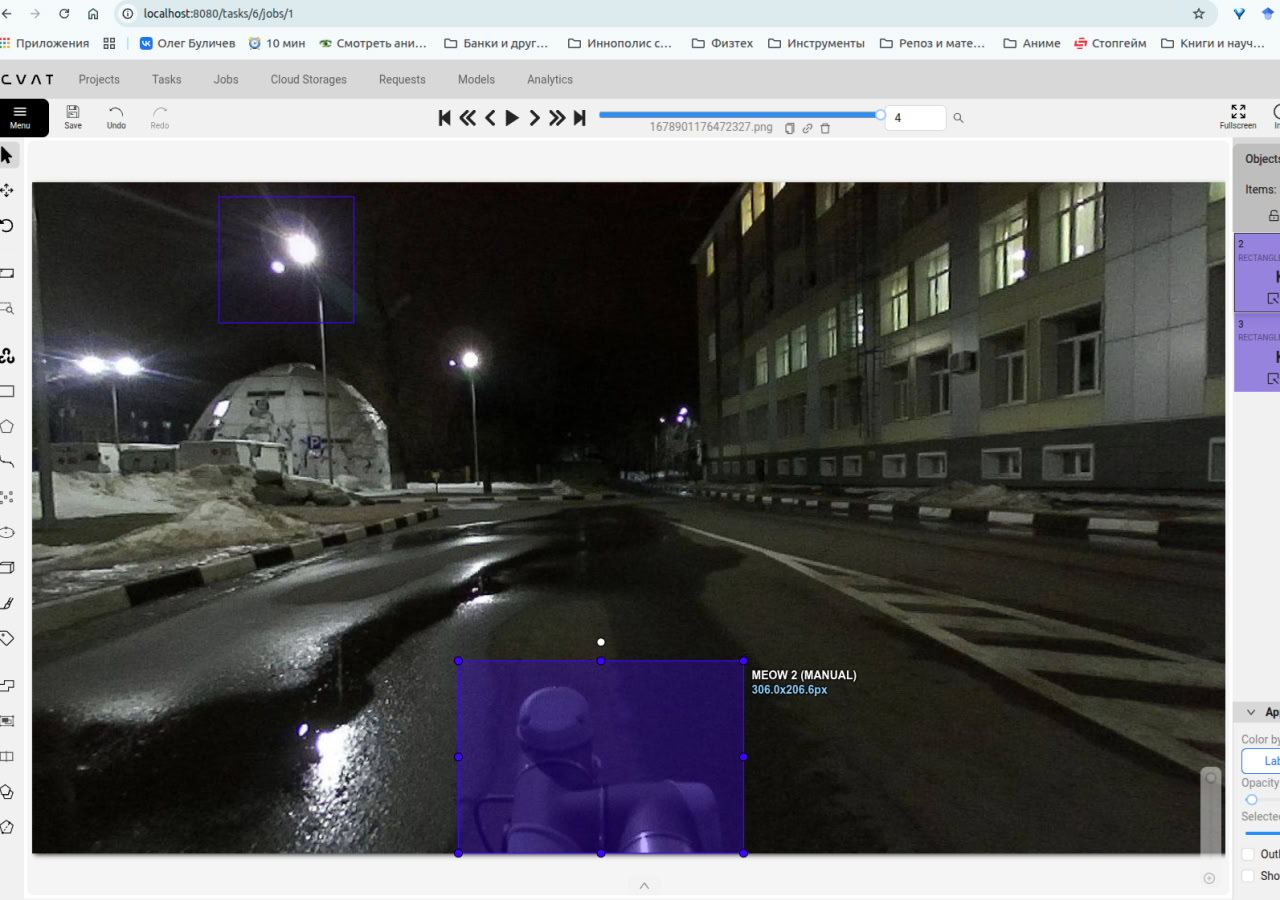
\includegraphics[height=4cm,width=1\textwidth,keepaspectratio]{cvat.png}
                % \caption{caption_name}
                \label{fig:cvat.png}
            \end{figure}
        \end{column}
    \end{columns}
\end{frame}

\begin{frame}[t]
    \frametitle{Supervisely}
    \begin{columns}
        \begin{column}{0.6\textwidth}
            \textbf{Core Features:}
            \begin{itemize}
                \item \textbf{Platform OS:} Comprehensive ecosystem for the entire CV lifecycle (Label $\rightarrow$ Train $\rightarrow$ Deploy).
                \item \textbf{App Ecosystem:} Hundreds of specialized apps for data cleaning, visualization, and model conversion.
                \item \textbf{Sensor Fusion:} Real-time synchronization between 2D images and 3D LiDAR point clouds.
                \item \textbf{Enterprise Scale:} Designed for heavy high-resolution imagery and complex ontologies.
            \end{itemize}
        \end{column}
        \begin{column}{0.4\textwidth}
            \begin{figure}[H]
                \centering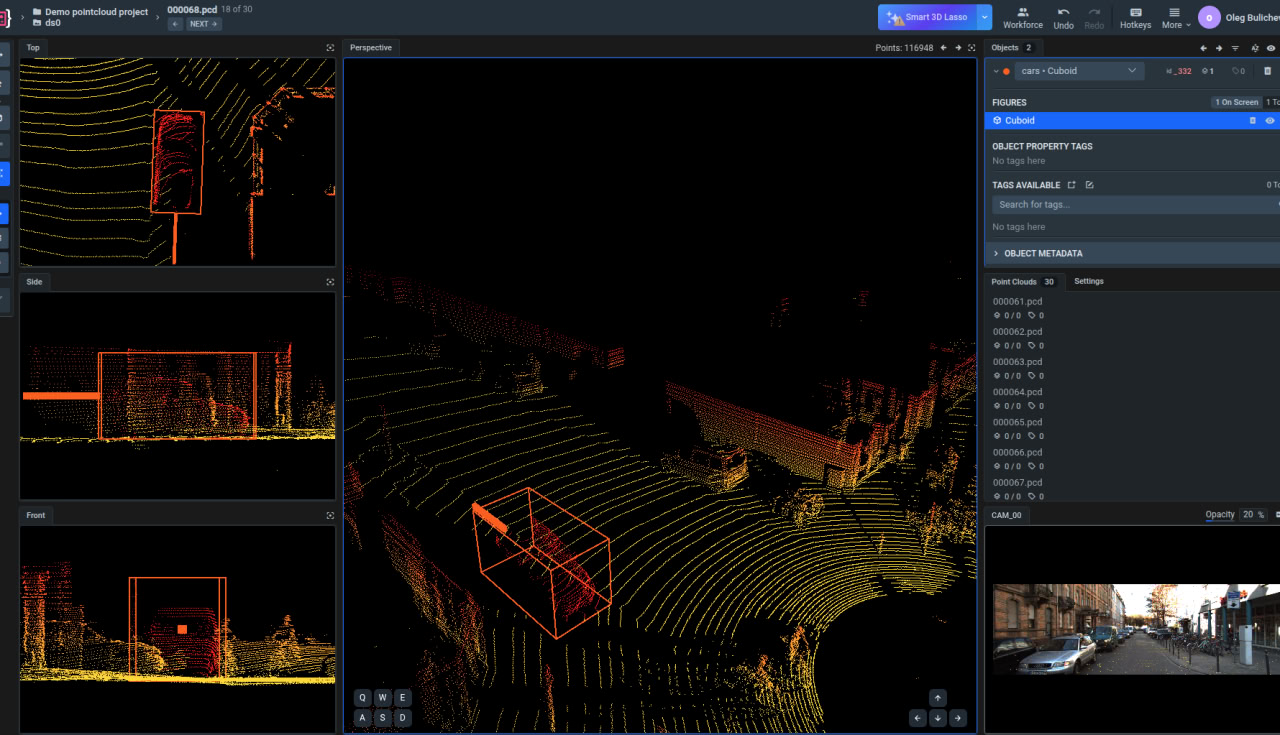
\includegraphics[height=4cm,width=1\textwidth,keepaspectratio]{supervisly.png}
                % \caption{caption_name}
                \label{fig:supervisly.png}
            \end{figure}
        \end{column}
    \end{columns}
\end{frame}

\begin{frame}[t]
    \frametitle{Roboflow}
    \begin{columns}
        \begin{column}{0.6\textwidth}
            \textbf{Core Features:}
            \begin{itemize}
                \item \textbf{Community Hub:} Access to the "Roboflow Universe" with 1M+ open-source datasets.
                \item \textbf{Web-First:} Simple, intuitive browser interface optimized for rapid prototyping.
                \item \textbf{Preprocessing:} Integrated tools for resizing, augmentations, and health checks.
                \item \textbf{Deployment:} One-click deployment to various edge devices via Roboflow Train.
            \end{itemize}
        \end{column}
        \begin{column}{0.4\textwidth}
            \begin{figure}[H]
                \centering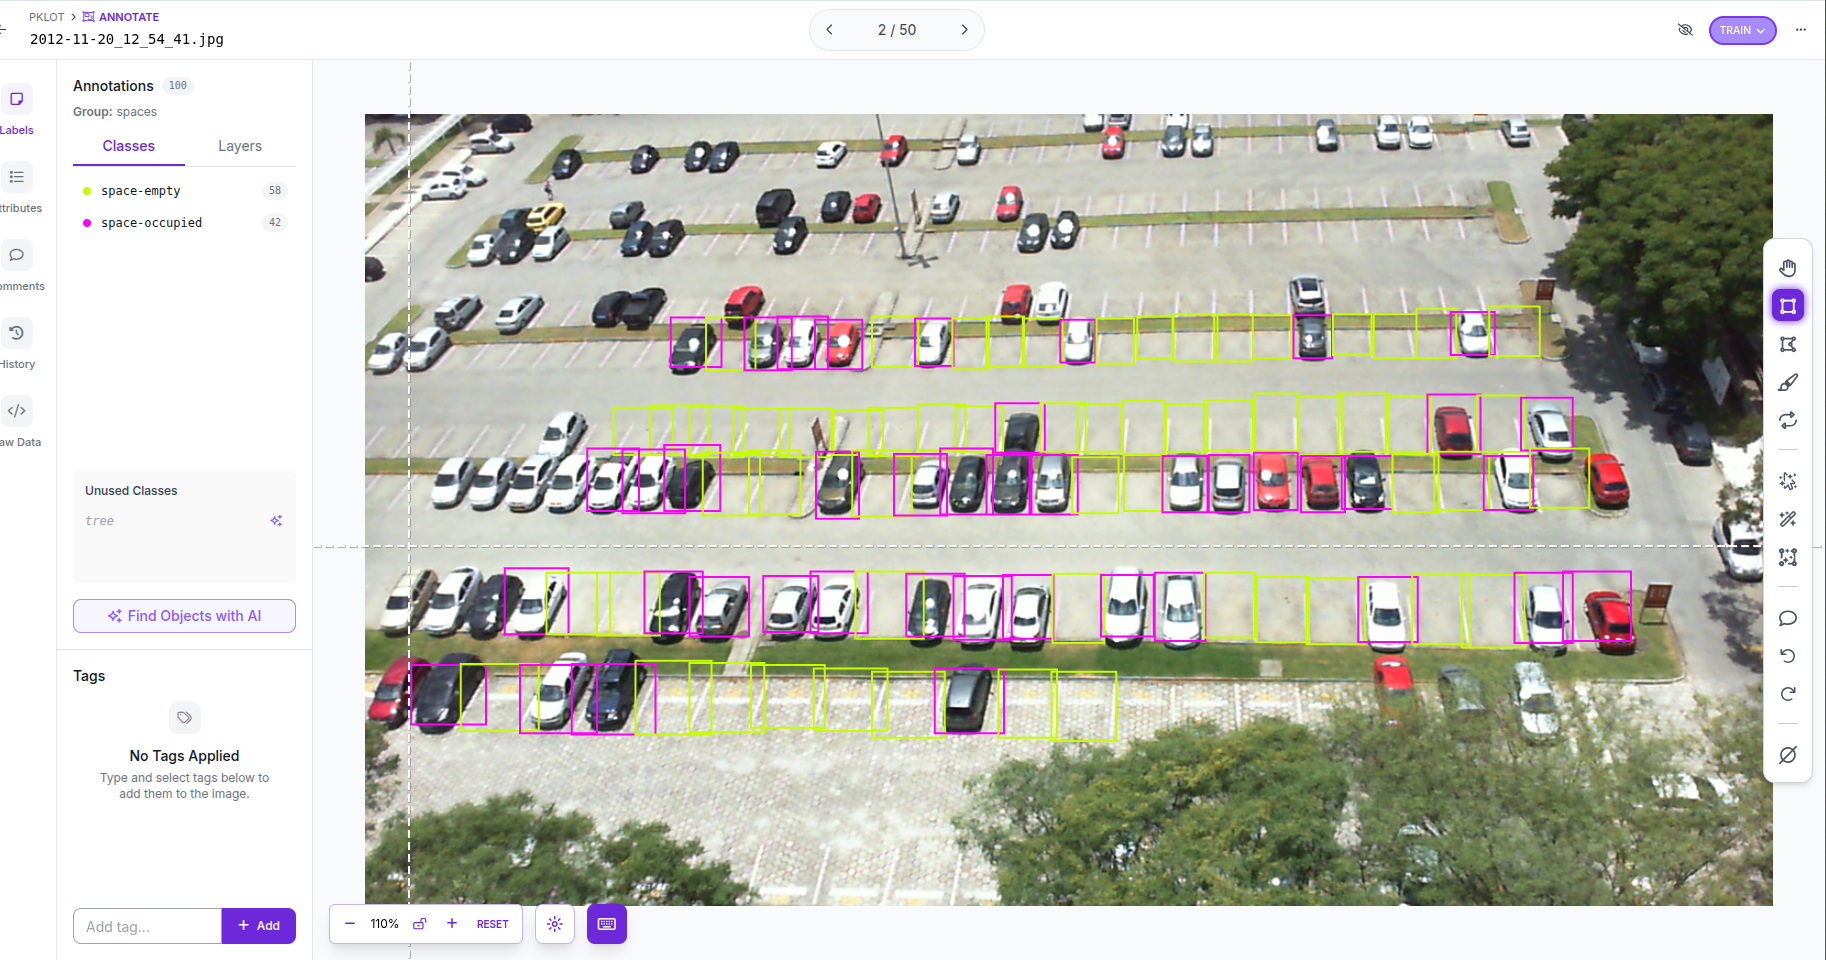
\includegraphics[height=4cm,width=1\textwidth,keepaspectratio]{roboflow.png}
                % \caption{caption_name}
                \label{fig:roboflow.png}
            \end{figure}
        \end{column}
    \end{columns}
\end{frame}

\begin{frame}[t]
    \frametitle{Point\_labeler}
    \begin{columns}
        \begin{column}{0.6\textwidth}
            \textbf{Core Features:}
            \begin{itemize}
                \item \textbf{LiDAR Focus:} Specifically designed for labeling millions of points in 3D scans.
                \item \textbf{Tile-based Rendering:} Loads scan tiles to handle massive KITTI point clouds efficiently.
                \item \textbf{OpenGL Shaders:} Uses modern graphics processing to render complex 3D scenes in real-time.
                \item \textbf{SemanticKITTI:} The primary tool used to create the landmark SemanticKITTI dataset.
            \end{itemize}
        \end{column}
        \begin{column}{0.4\textwidth}
            \begin{figure}[H]
                \centering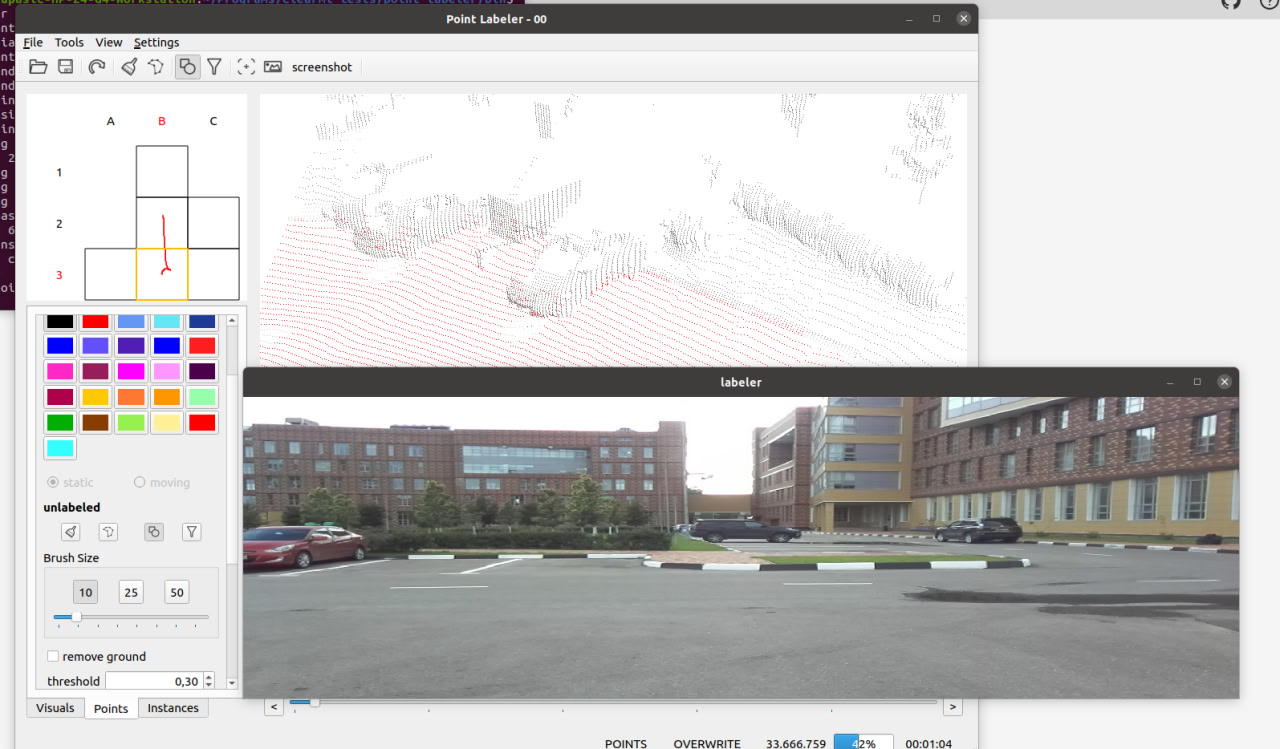
\includegraphics[height=4cm,width=1\textwidth,keepaspectratio]{point_labeler.png}
                % \caption{caption_name}
                \label{fig:point_labeler.png}
            \end{figure}
        \end{column}
    \end{columns}
\end{frame}

\begin{frame}[t]
    \frametitle{References}
    \begin{itemize}
        \item \href{https://www.cvat.ai/}{CVAT: Leading Data Annotation Platform}
        \item \href{https://supervisely.com/}{Supervisely: Computer Vision Platform}
        \item \href{https://roboflow.com/}{Roboflow: Computer Vision Datasets \& Models}
        \item \href{https://github.com/jbehley/point_labeler}{GitHub: point\_labeler tool}
        \item \href{https://blog.deepschool.ru/cvat-guide/}{CVAT Full Guide — Data Light}
    \end{itemize}
\end{frame}
\begin{frame}[t]
    \frametitle{The Landscape of Data Versioning}
    Modern MLOps relies on three primary tools for managing datasets:
    \begin{itemize}
        \item \textbf{DVC (Data Version Control):} Acts as a Git extension, storing lightweight \texttt{.dvc} pointers in Git while physical data resides in remote storage like S3.
        \item \textbf{Hugging Face Datasets:} A specialized library for NLP, Vision, and Audio, integrated with the HF Hub for sharing and versioning.
        \item \textbf{ClearML Data:} A module of the ClearML platform that manages data independently of code, adhering to the "Data is not Code" philosophy.
    \end{itemize}
\end{frame}

\begin{frame}[t]
    \frametitle{ClearML Data: Structure and Philosophy}
    \begin{itemize}
        \item \textbf{Philosophy:} ClearML believes data progress is often non-linear and should not be stored in a Git tree.
        \item \textbf{Everything is a Task:} In the ClearML ecosystem, datasets, experiments, and pipelines are all handled as the same object type: a \textbf{Task}.
        \item \textbf{Decoupling:} Data management is handled via the \texttt{clearml-data} CLI or the \texttt{clearml.Dataset} Python SDK.
        \item \textbf{Single Source of Truth:} The ClearML Server tracks experiment runs and dataset versions over time for exact recreation.
    \end{itemize}
\end{frame}

\begin{frame}[t]
    \frametitle{Key Concepts of ClearML Data}
    \begin{itemize}
        \item \textbf{Accessibility:} Ensures data is accessible from any machine (local, cloud, or remote agents).
        \item \textbf{Ancestry/Lineage:} Automatically tracks where specific parts of data came from through parent-child relationships.
        \item \textbf{Differentiable Storage:} Only uploads the \textbf{delta} (differences) between a new version and its parent, saving bandwidth and space.
        \item \textbf{Immutability:} Once a dataset version is "Finalized," it is locked to ensure reproducibility.
    \end{itemize}
\end{frame}

\begin{frame}[t]
    \frametitle{Dataset Management via CLI}
    The \texttt{clearml-data} utility allows for quick operations:
    \begin{itemize}
        \item \textbf{Creation:} \texttt{clearml-data create --project "Proj" --name "DS"}.
        \item \textbf{Adding Files:} \texttt{clearml-data add --path ./local\_folder} (recursively adds all files).
        \item \textbf{Finalizing:} \texttt{clearml-data close} (uploads files and locks the version as "Final").
        \item \textbf{Synchronization:} \texttt{clearml-data sync --folder ./data} (combines create, add, and upload in one step).
    \end{itemize}
\end{frame}

\begin{frame}[t]{ClearML Dataset Lineage}
\framesubtitle{}
    \vspace{-0.6cm}
    \begin{figure}[H]
        \centering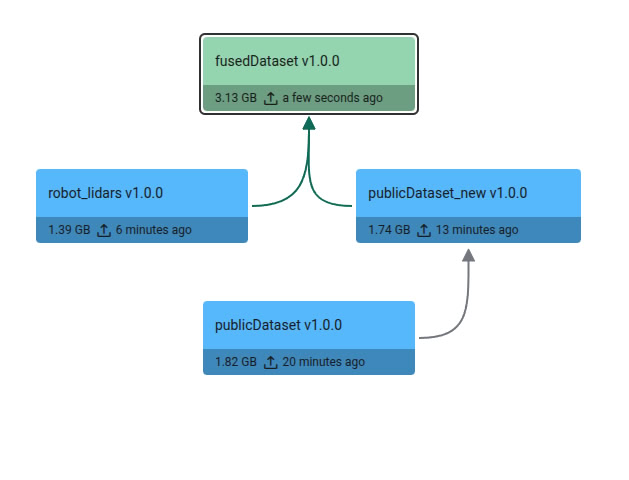
\includegraphics[height=6cm,width=1\textwidth,keepaspectratio]{clearml_lineage.png}
        \label{fig:clearml_lineage.png}
    \end{figure}
\end{frame}

\begin{frame}[t]
    \frametitle{Reproducibility: Linking Data to Tasks}
    \begin{itemize}
        \item \textbf{Automatic Connection:} When a training task uses \texttt{Dataset.get()}, ClearML automatically records the Dataset ID in the task's configuration.
        \item \textbf{Traceability:} Users can see exactly which version of a dataset produced which model in the Web UI.
        \item \textbf{Collaboration:} Team members can use \texttt{get\_local\_copy()} to work with identical data slices, ensuring consistent results across the team.
    \end{itemize}
\end{frame}

\begin{frame}[t]
    \frametitle{References}
    \begin{itemize}
        \item \href{https://blog.deepschool.ru/data/clearml-data-management/}{ClearML Data Management — DeepSchool}
        \item \href{https://clear.ml/docs/latest/docs/clearml_data/clearml_data_interface/}{ClearML Data Interface Documentation}
        \item \href{https://huggingface.co/docs/datasets/index}{Hugging Face Datasets Documentation}
        \item \href{https://dvc.org/doc/use-cases/versioning-data-and-models}{DVC: Versioning Data and Models}
        \item \href{https://youtube.com/playlist?list=PLp_9id_N7_QN0XyV_9I-j24DAn7Y_v-m_}{ClearML Official YouTube: Getting Started Series}
    \end{itemize}
\end{frame}



\fbckg{fibeamer/figs/last_page.png}
\frame[plain]{}

\end{document}
